\documentclass{beamer}
%
% Choose how your presentation looks.
%
% For more themes, color themes and font themes, see:
% http://deic.uab.es/~iblanes/beamer_gallery/index_by_theme.html
%

\mode<presentation>
{
  \usetheme{default} % or try Darmstadt, Madrid, Warsaw, ...
  \usecolortheme{default} % or try albatross, beaver, crane, ...
  \usefonttheme{serif} % or try default, structurebold, ...
  \setbeamertemplate{navigation symbols}{}
  \setbeamertemplate{caption}[numbered]
}
\newcommand*\vf[1]{\mathbf{#1}}
\usepackage[english]{babel}
\usepackage[utf8x]{inputenc}
\usepackage{amsmath,mathtools,esint,bm}
\usepackage{todonotes}
\usepackage{blindtext}
\usepackage[font=scriptsize]{caption}
\usepackage[version=3]{mhchem}
\newcommand{\mick}[1]{\textcolor{red}{#1}}

\AtBeginSection[]{
  \begin{frame}
  \vfill
  \centering
  \begin{beamercolorbox}[sep=8pt,center,shadow=true,rounded=true]{title}
    \usebeamerfont{title}\insertsectionhead\par%
  \end{beamercolorbox}
  \vfill
  \end{frame}
}

\title[]{Charge density waves in Bi$_2$Sr$_{2-x}$La$_x$CuO$_{6 + \delta}$}
\author{Mick Krongchon}
\institute{University of Illinois at Urbana-Champaign}
\date{\today}

\begin{document}

\begin{frame}
\titlepage
\end{frame}
% Hi everyone, today I'm gonna be talking about charge density waves in this material which we're just gonna call BSCCO
% Well, in my last two presentations, it was me trying to understand what charge density wave really is, but I didn't really succeed
% But this time, I'm just gonna report what people have found

\begin{frame}
\centering
\textit{intentionally left blank}
\end{frame}
% CRITIQUE: Motivation too broad, Outline too general

\begin{frame}{Outline}
\begin{itemize}
\item Motivation
\item Observations of the charge density wave(s) in various doping
\item Conclusion
\end{itemize}
\end{frame}
% This is the outline of my presentation

\begin{frame}{Goal: Mechanism for high-$T_\text{c}$ superconductivity (SC)}
\begin{itemize}
\item $T$ and magnetic field dependence show competition between charge density wave (CDW) and SC in YBCO by J. Chang et~al (2012)
\end{itemize}
\begin{figure}
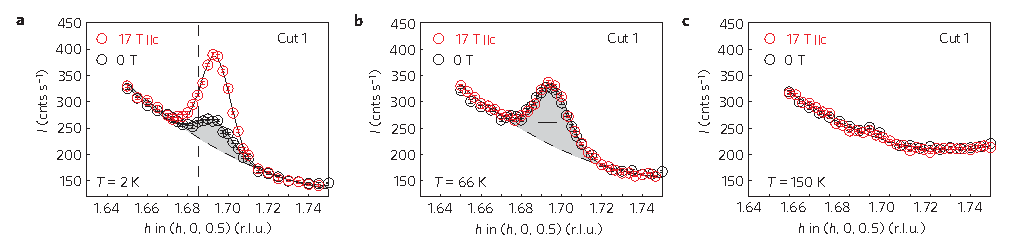
\includegraphics[width=\textwidth]{figs/chang_1.pdf}
\caption*{Scans along $(h, 0, 0.5)$ for magnetic fields and temperature: \\(a) $T < T_c$, (b) $T_c < T < T_{\text{CDW}}$, (c) $T > T_{\text{CDW}}$}
\end{figure}
\end{frame}
% We want to understand high temperature superconductivity
% And last time, I showed the evidence of competition between CDW and SC in YBCO by J. Chang in 2012
% So, just to recap: the CDW signal increases when SC is suppressed
% But today we're gonna look into BSCCO because CDW is pretty common among cuprates, and doping in BSCCO can be tuned over a wide range

\begin{frame}{CDW in the underdoped and optimally doped BSCCO}
\begin{itemize}
\item Y. Y. Peng et~al. (2016): RIXS for UD15K (p = 0.115) and OP33K (p = 0.16)
\end{itemize}
\begin{figure}
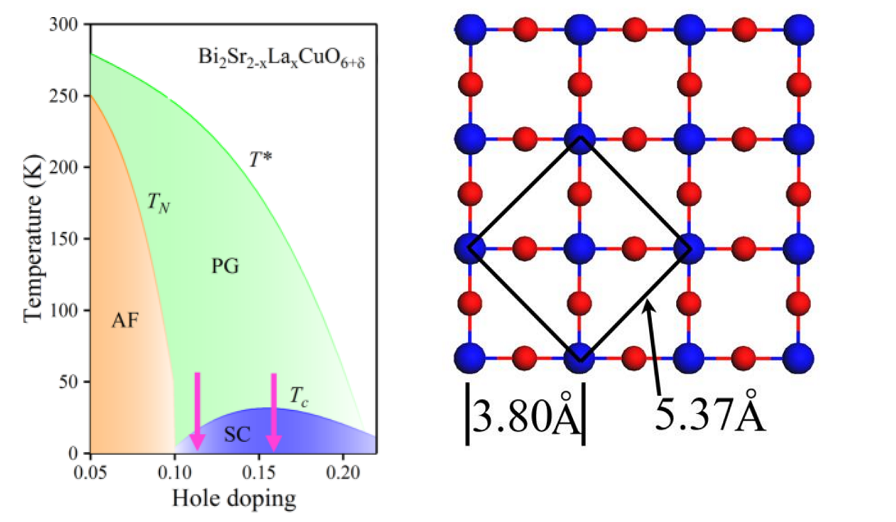
\includegraphics[width=3.5in]{figs/1a_lattice.png}
\caption*{(\textbf{Left}) Phase diagram of Bi2201. (\textbf{Right}) Lattice image of the CuO$_2$ plane}
\end{figure}
\end{frame}
% So, the experiment I want to talk about was done by Ying Ying Peng, who is now a post-doc from Peter Abbamonte group, and other people.
% For Bi2201, previous RIXS results show no evidence of CDW at optimal doping (in contrast to the ARPES results)
% That's another motivation to do this experiment
% And, the two dopings that they did were UD15K, which is a shorthand for underdoped which has Tc = 15K, and OP33K

\begin{frame}{CDW modulates only along Cu-O bonds}
\begin{itemize}
\item Find $q_\text{CDW}$ from RIXS energy/momentum intensity maps
\item $q_\text{CDW} = 0.26$ for UD15K and $q_\text{CDW} = 0.23$ for OP33K
\end{itemize}
\begin{figure}
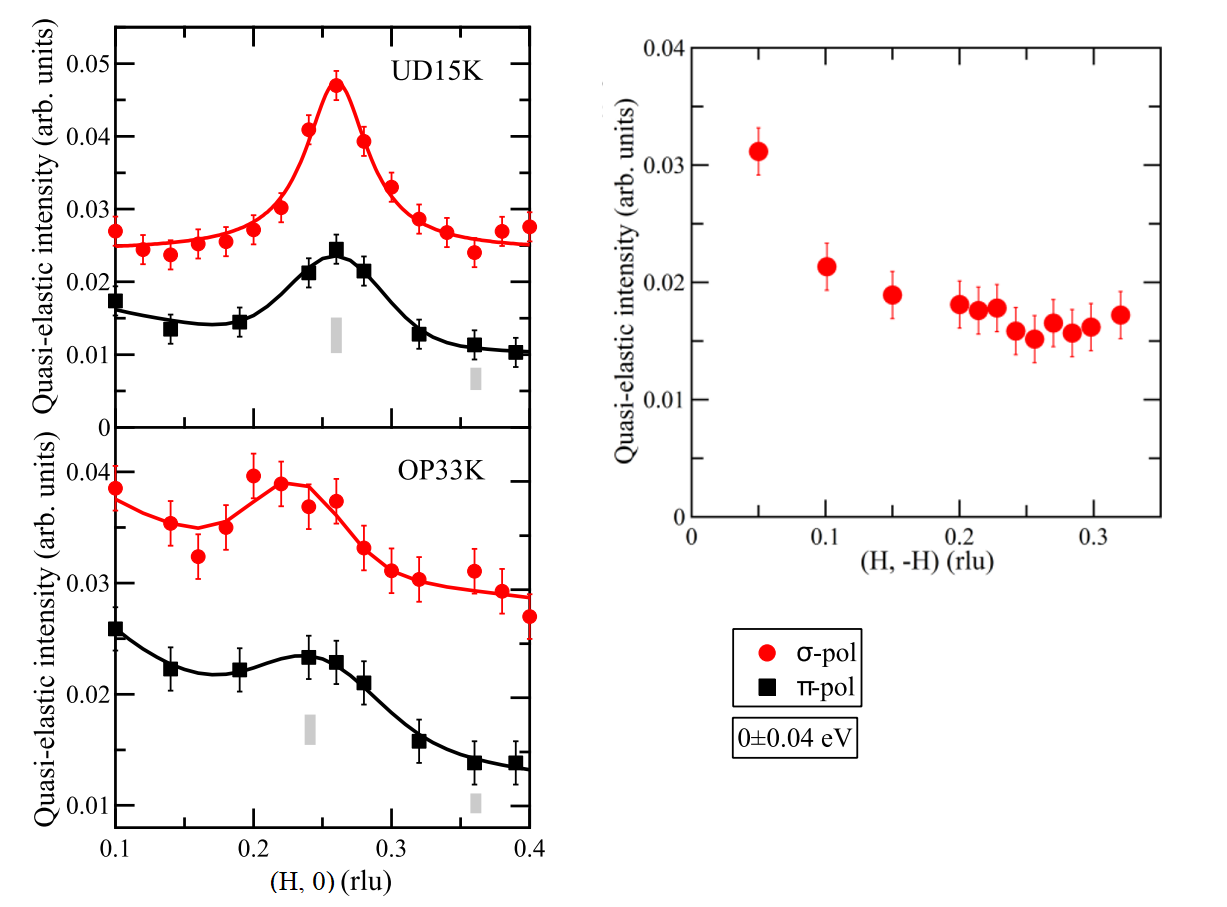
\includegraphics[width=3.2in]{figs/2ab_4a.png}
\caption*{Intensity along (0,0)-(0.5,0) (\textbf{left}) and along (0,0)-(0.5,-0.5) (\textbf{right}) for UD15K}
\end{figure}
\end{frame}
% So, when we do the RIXS experiment, we should get the energy/momentum intensity maps, which I do not show
% And, from there, we can find q_CDW by analyzing the peaks from the cut, in this case E = 0 \pm 0.04 ev
% On the left, we can see the peak, and they call this peak REXS
% The intensity doesn't show any peak.
% This confirms that CDW is only along Cu-O bonds.

\begin{frame}{Temperature dependence}
\begin{itemize}
\item CDW signal can be seen at 20~K and becomes sharper at 33~K (similar to YBCO)
\item Confirms the competition between CDW and SC
\end{itemize}
\begin{figure}
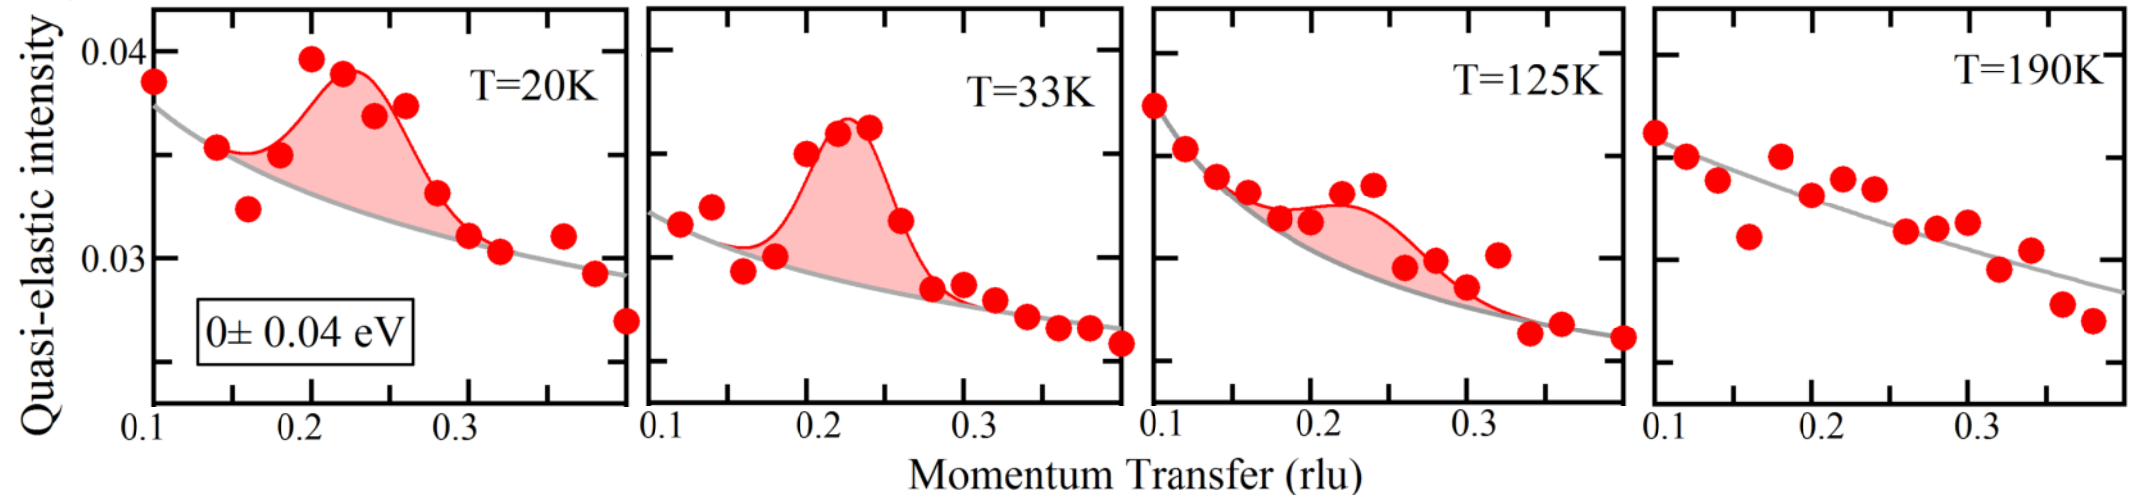
\includegraphics[width=4.2in]{figs/5e.png}
\caption*{Temperature dependence across $T_c = 33~\mathrm{K}$ and $T^{*} = 160~\mathrm{K}$ for OP33K}
\end{figure}
\end{frame}


\begin{frame}{What about the overdoped region?}
\begin{itemize}
\item No direct evidence of CDW in overdoped cuprates even though it was predicted in theory
\item Y. Y. Peng et~al. (2018): RIXS for Bi2201 in OD17K ($p = 0.205$), OD11K ($p = 0.215$), and OD0K ($p = 0.23$)
\end{itemize}
\begin{figure}
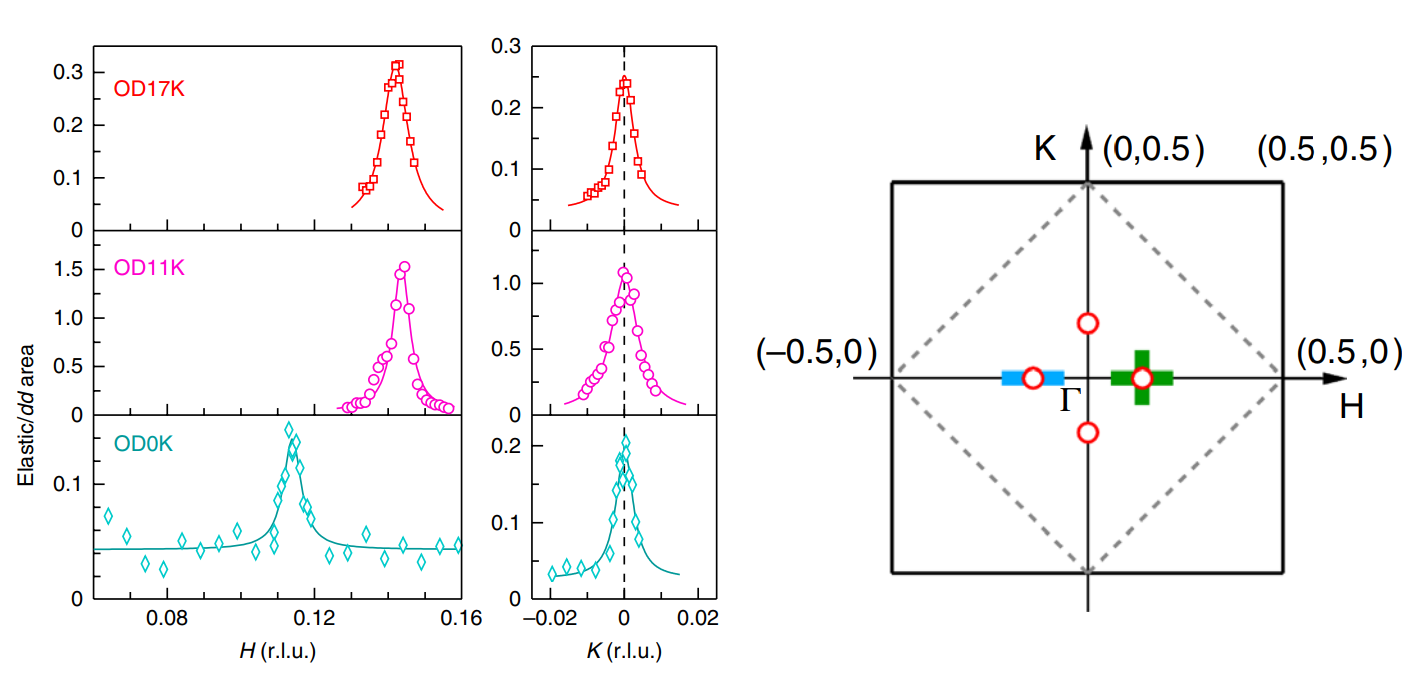
\includegraphics[width=4in]{figs/2018_2b.png}
\caption*{REXS intensity along $H$ and $K$ at different doping levels}
\end{figure}
\end{frame}

\begin{frame}{Small temperature dependence}
\begin{itemize}
\item CDW can still occur well above 250~K (even in the absense of the pseudogap)
\end{itemize}
\begin{figure}
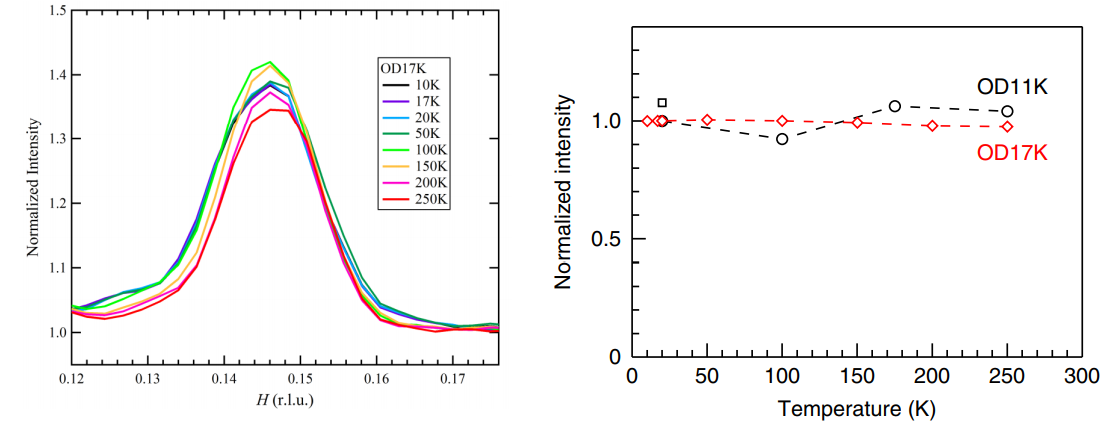
\includegraphics[width=4in]{figs/2018_s10_3d.png}
\caption*{(\textbf{Left}) Intensity scans at different temperatures in OD17~K. (\textbf{Right}) Temperature dependence in OD11K and OD17K (normalized to at 20~K)}
\end{figure}
\end{frame}

\begin{frame}{Do REXS peaks actually arise from CDW?}
\begin{itemize}
\item Charge scattering (no spin-flip) conserves the photon polarization
\item Bi2201 has only one Cu site contributing to the x-ray absorption spectrum, and can be assigned to CDW in CuO$_2$ planes
\end{itemize}
\begin{figure}
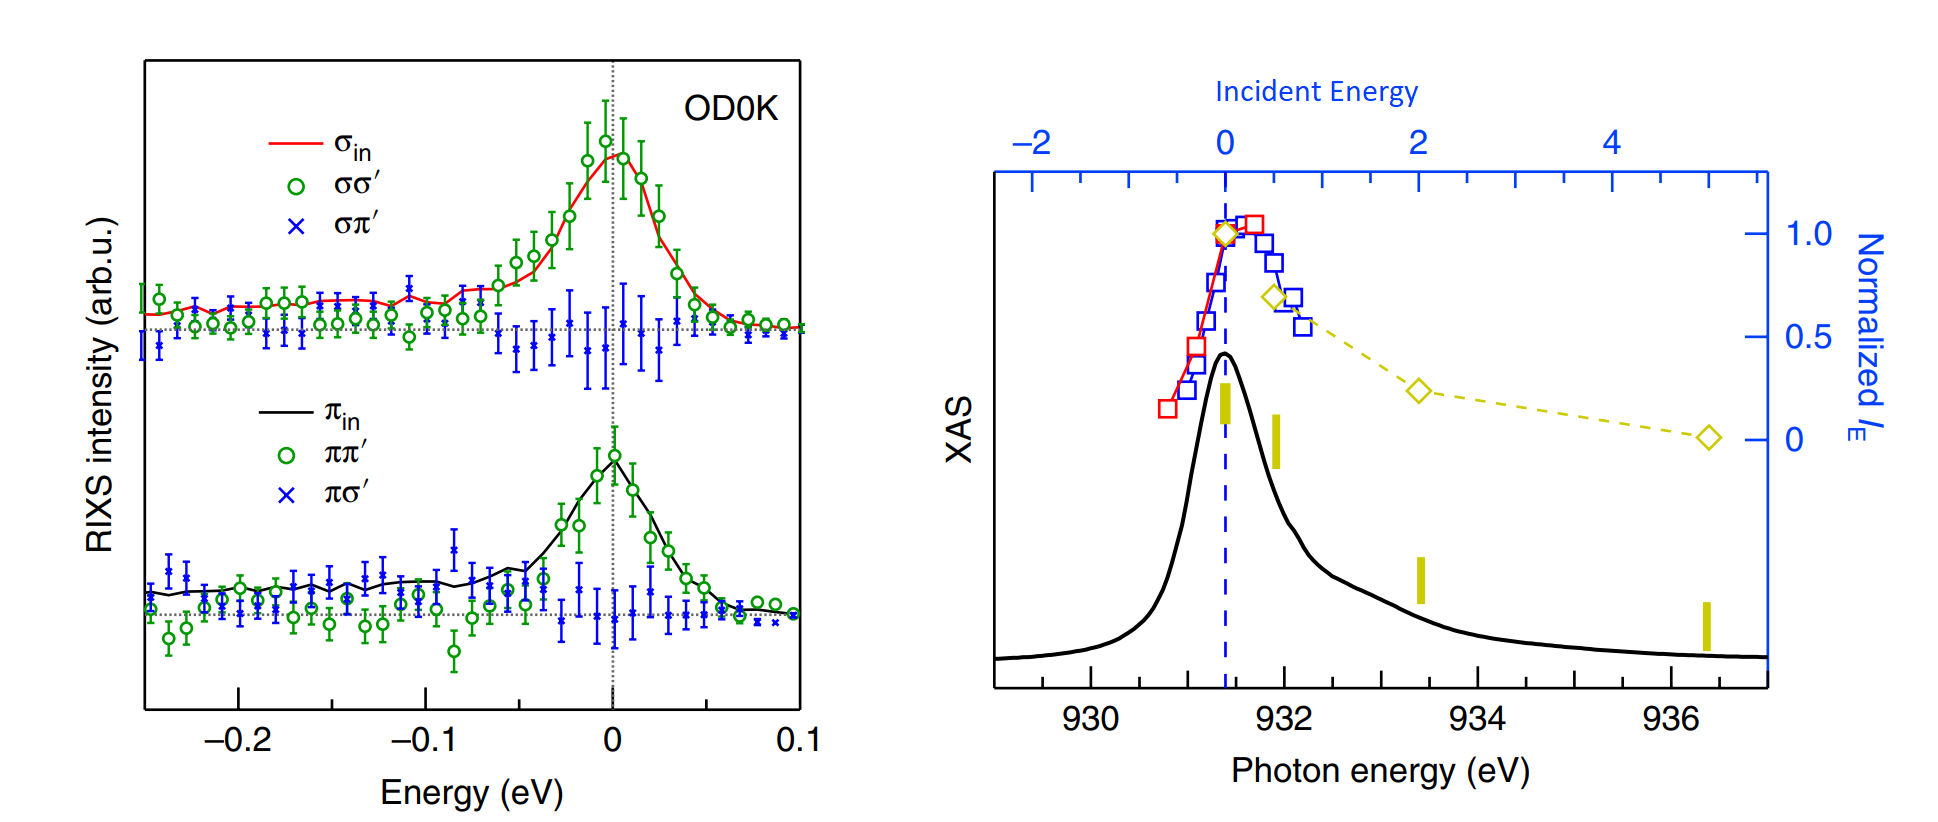
\includegraphics[width=4in]{figs/2018_2c_3a.png}
\caption*{(\textbf{Left}) Polarization-resolved measurements for OD0K at $H = 0.115$. (\textbf{Right}) (Left and bottom axes) X-ray absorbtion spectrum of OD17K. (Right and top axes) Incident energy dependence of the REXS intensity}
\end{figure}
\end{frame}

\begin{frame}{Doping dependence}
\begin{itemize}
\item The peak intensity is higher in the overdoped region
\item The correlation lengths $\xi$ are comparable to LCO and YBCO
\end{itemize}
\begin{figure}
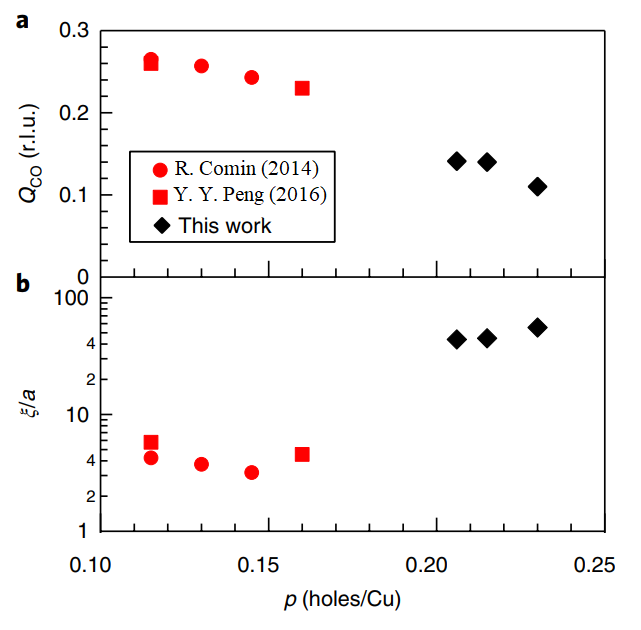
\includegraphics[width=2.5in]{figs/2018_4.png}
\caption*{Doping dependence of $q_\text{CDW}$ (\textbf{a}) and correlation length (\textbf{b})}
\end{figure}
\end{frame}

% not sure why they didn't do overdoped in previously
% they call this peak REXS

\begin{frame}{Need to revisit existing theories}
\begin{itemize}
\item Charge instabilities are related to the van Hove singularity and Fermi surface nesting, (which are absent in this experiment)
\item CDWs arise from the pseudogap phase (relevant to only the underdoped region)
\end{itemize}
\end{frame}

\begin{frame}{Summary}
\begin{itemize}
\item CDW can exist well above optimal doping
\end{itemize}
\end{frame}

% \begin{frame}{Why care about the Fermi surface (FS)?}
% \begin{itemize}
%   \item The origins of various phenomena can be traced back to the FS shape
%   \item Helps understand the mechanism of charge density waves
%   \item Can be experimentally measured
%   % \item

%   % \item The Fermi surface is the surface in reciprocal space which separates occupied from unoccupied electron states at zero temperature


% % \item CDW is a phase transition at low $T$
% % \item Metals undergo a phase transition when they are cooled
% % \item i.e. Iron and nickel become FM. Lead and Al become superconductors
% % \item Since 1970s, many layered materials have been found to undergo this phase transition
% % \item Want to study CDW
% \end{itemize}
% \end{frame}

% \begin{frame}{How to calculate the FS}
% \begin{itemize}
% \item Calculate the band structure using some method (by hand, tight binding, DFT, HF, etc.)
% \item Know the Fermi energy, $E_F$, from the number of electrons
% \item FS is a plot of constant energy with $E = E_F$
% \end{itemize}
% \end{frame}

% \begin{frame}{1D Fermi gas}
% \begin{itemize}
% \item The Fermi energy is given by
% \begin{align}
% E_F = \frac{\hbar^2}{2 m}\left(\frac{\pi n_F}{L}\right)^2 = \frac{\hbar^2}{2 m}\left(\frac{\pi N}{2 L}\right)^2,
% \end{align}
% because orbitals must be filled up to $n_F$ for $N$ electrons given by
% \begin{align}
% N = 2 \times \frac{1}{2} \times 2 n_F = 2 n_F,
% \end{align}
% where $n_F$ is the radius of an integer-space ``sphere''.
% \item The Fermi surface is points at $\pm \pi N / 2 L$
% \end{itemize}
% \end{frame}

% \begin{frame}{This FS geometry leads to a divergent response}
% \begin{itemize}
% \item The rearrangement of the charge density in a potential $\phi(\vf{r})$ can be written as
% \begin{align}
% \rho(\vf{q}) = \chi(\vf{q}) \phi(\vf{q}),
% \end{align}
% where $\chi(\vf{q})$ is the Lindhart function given in $d$ dimensions by
% \begin{align}
% \chi(\vf{q}) = \frac{1}{(2 \pi)^d} \int \frac{f_k - f_{k + q}}{E_k - E_{k + q}} d \vf{k},
% \end{align}
% which in the 1D case, evaluates to
% \begin{align}
% \chi(q) = \frac{k_F}{\pi E_F q}\ln{\left|\frac{q + 2k_F}{q - 2k_F}\right|}.
% \end{align}
% \end{itemize}
% \end{frame}

% \begin{frame}{An external perturbation leads to a divergent charge density}
% \begin{itemize}
% \item Causes a charge density redistribution
% \item The divergence at $q = 2 k_F$ is called \textbf{perfect nesting}
% \begin{figure}
% 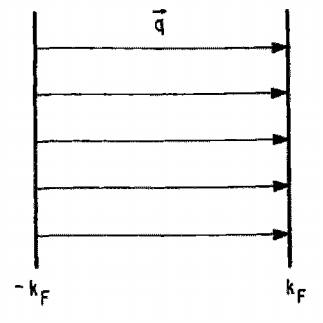
\includegraphics[width=1.5in]{figs/1d_nesting.png}
% \caption{\label{fig:1d_nesting} Fermi surface topology for a 1D electrong gas, The arrows indicate pairs of states, differing by the
% wavevector $q = 2 k_F$.}
% \end{figure}
% \end{itemize}
% \end{frame}

% \begin{frame}{The rearrangement of atoms and charges results in a lower energy}
% \begin{itemize}
% \item The new lattice has a period of $2a$
% \item The $\vf{k}$ vector now range from $-\pi / 2a$ to $\pi / 2a$
% \item The band is now split into two bands
% \item The atomic motion is causing the electrons to reconfigure
% \item This is called a \textbf{charge density wave (CDW)}
% \begin{figure}
% 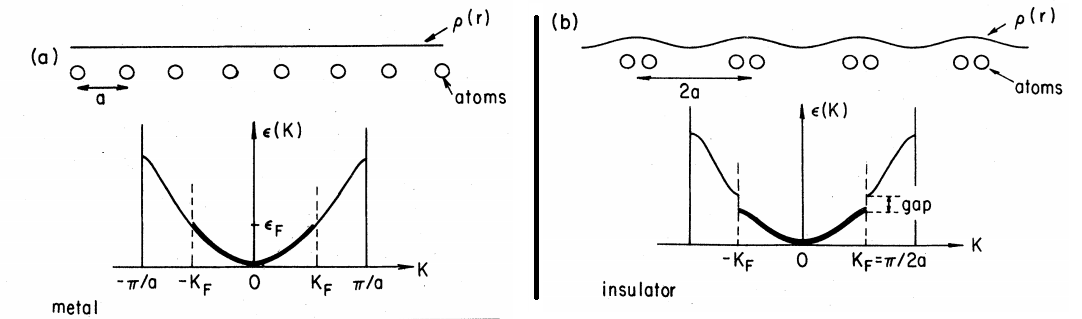
\includegraphics[width=3.5in]{figs/gap.png}
% \caption{\label{fig:gap} Peierls distortion in a one-dimensional metal with a half-filled band: (a) undistorted metal, (b) Peierls insulator.}
% \end{figure}
% % Imagine a line of atoms on equally-spaced positions sharing their electrons to make a conduction band.
% % You have exactly one electron per atom.
% % And, the k-vectors range from −π/a to π/a.
% %% The electrons are split in spin 50/50, so you get filling of the states in the first band up to exactly ±π/2a, and that's the Fermi surface (two points). This is called a half-filled band, since the states are filled duplicately until the exact half-way point.
% % But if there's electron-electron or electron-phonon interaction
% % period of the lattice is given by lambda = pi / k_F
% \end{itemize}
% \end{frame}

% \begin{frame}{What about superconductivity (SC)?}
% \begin{itemize}
% \item In 1954, Fröhlich attempted to explain SC using CDW (even before the BCS theory)
% \item His model was not wrong but incomplete (did not explain the Meissner effect)
% \item SC occurs in proximity to CDW
% \item Question: Is this significant (SC emerges from CDW) or trivial (the electronic structure independently favors both)?
% \end{itemize}
% \end{frame}

% \begin{frame}{Evidence of the competition between SC and CDW}
% \begin{itemize}
% \item J. Chang et al's \textit{Direct observation of competition between superconductivity and charge density wave order in YBa$_2$Cu$_3$O$_{6.67}$} (2012)
% \item Want to measure when such states exist
% \item X-ray diffration in magnetic fields up to 17~T with the hole concentration per Cu $p = 0.12$
% \end{itemize}
% \end{frame}

% \begin{frame}{Results: The CDW signal increases when SC is suppressed at $H = 17~T$ and $T = 2~K$}
% \begin{itemize}
% \item The charge modulation has two field- and temperature-independent wave vectors $\vf{q}_{\text{CDW}} = \vf{q}_1 = (\delta_1, 0, 0.5)$ and $\vf{q}_2 = (0, \delta_2, 0.5)$ where $\delta_1 = 0.305$ and $\delta_2 = 0.315$
% % \item The CDW gives rise to peaks the at $\vf{Q} = (2 \pm \delta_1, 0, 0.5)$
% \end{itemize}
% \begin{figure}
% 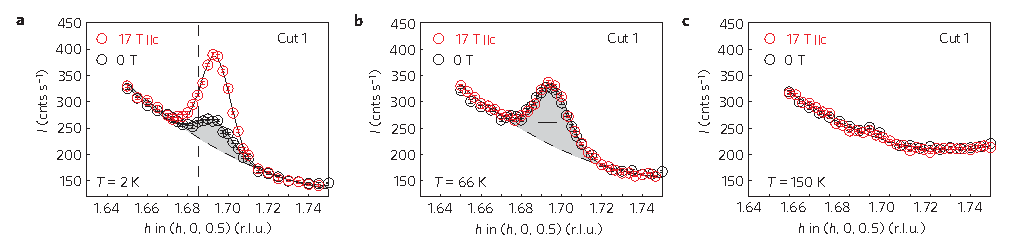
\includegraphics[width=\textwidth]{figs/chang_1.pdf}
% \caption{\label{fig:chang_1} Scans along $(h, 0, 0.5)$ for temperature and magnetic fields: (a) $T < T_c$, (b) $T_c < T < T_{\text{CDW}}$, (c) $T > T_{\text{CDW}}$}
% \end{figure}
% \end{frame}

% \begin{frame}{The FS of YBCO consists of bonding and anti-bonding sheets (according to ARPES and LDA)}
% \begin{itemize}
% \item The electronic states connected by $\vf{q}_{\text{CDW}}$ are the bonding bands near the zone boundary
% \item The states lie near the maxima of the superconducting gap
% \item This (probably) means the CDW state is competing with SC for FS
% \begin{figure}
% 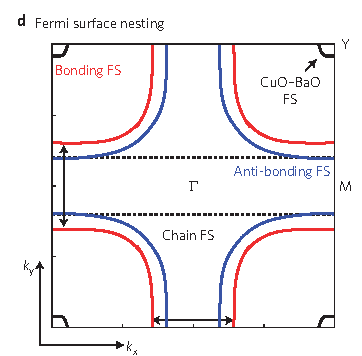
\includegraphics[width=1.5in]{figs/chang_3.pdf}
% \caption{\label{fig:chang_3} FS of YBCO}
% \end{figure}
% \end{itemize}
% \end{frame}

% \begin{frame}{Implications for the phase diagrams}
% \begin{itemize}
% \item A Landau theory: $T_c$ is suppressed in the presence the CDW
% \item $T_{\text{CDW}}$ corresponds with $T_\text{H}$, where Hall effect measurements suggest FS reconstruction
% \item A CDW that breaks translational symmetry explains the mechanism of FS reconstruction
% \end{itemize}
% \begin{figure}
% \includegraphics[width=1.5in]{figs/chang_4.pdf}
% \caption{\label{fig:chang_4} Doping dependence of several ordering temperatures}
% \end{figure}
% \end{frame}

% \begin{frame}{Conclusion}
% \begin{itemize}
% \item The Fermi surface nesting results in a diverging charge distribution
% \item The atomic distortion and electron rearrangement to the lower energy are called \textbf{charge density wave}
% \item The charge density wave signal increases when the superconductivity is suppressed
% \end{itemize}
% \end{frame}

% \begin{frame}{Peierls' picture: 1D chain}
% \begin{itemize}
% % \item In 1930s, Peierls described the instability in a 1D chain of equally spaced atoms
% % \item The only zero energy transition is from $k_F$ to $-k_F$, % where $k_F$ is the Fermi wave number
% \item The Fermi points are at $k_F = \pm \pi / 2 a$ % connected by a vector $q = 2 k_F$
% % \item The disturbance with $q = 2 k_F$ changes spacing to $2 a$
% \item Gap occurs at $k = \pm \pi / 2 a$ when $T < T_c$
% \item Metal-to-insulator transition at $T_c$ is called \textbf{Peierls' transition}

% \end{itemize}
% \end{frame}

% \begin{frame}{Free electron gas model}
% \begin{itemize}
% \item \textbf{Lindhard response function} $\chi(q)$ describes free electron gas' response
% \item 1D electron gas is unstable
% % \begin{figure}
% % 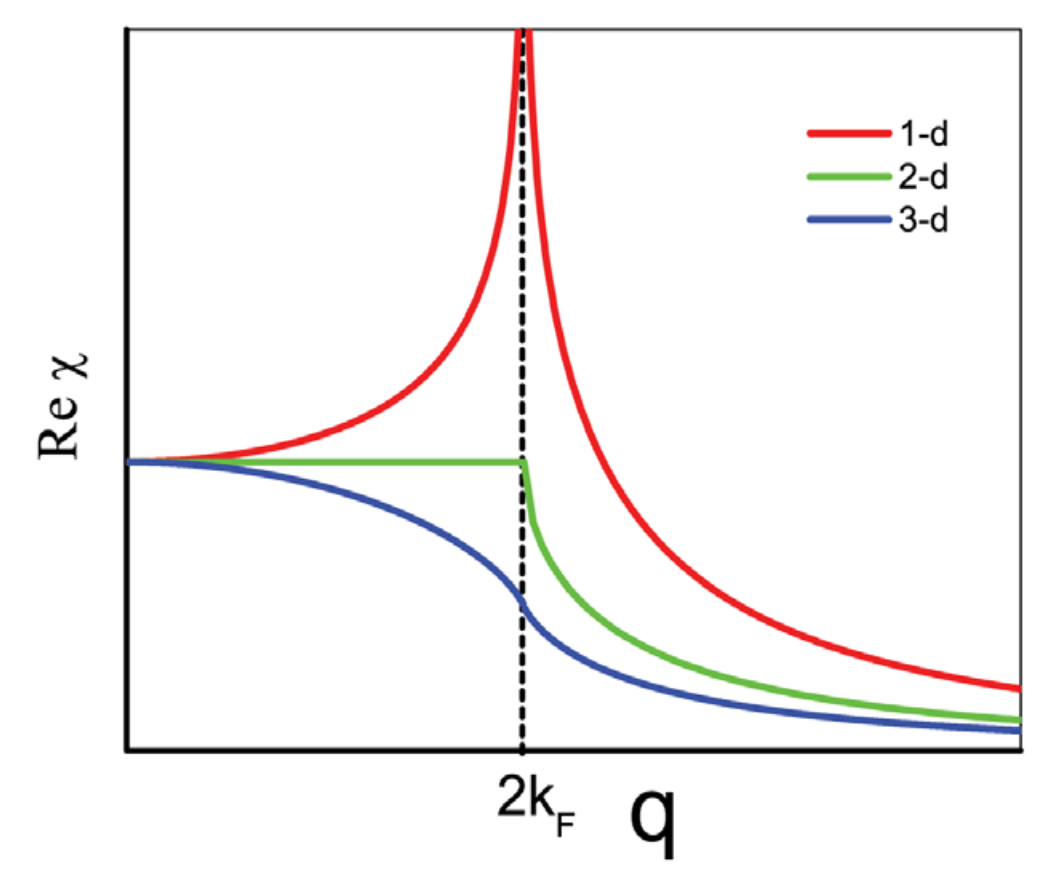
\includegraphics[width=2.5in]{figs/lindhart.png}
% % \caption{\label{fig:lindhart} Real part of Linhard function for 1D, 2D and 3D free electron gas models}
% % \end{figure}
% \end{itemize}
% \end{frame}

% \begin{frame}{Kohn anomaly}
% \begin{itemize}
% \item In 1959, Kohn: The excitations at $2 k_F$ will screen any lattice motion with this wave vector
% \item The phonon modes near $2 k_F$ will drop to a lower energy
% \item This is called \textbf{phonon softening}
% %  This strong renormalization of the phonon due to interactions with an electron system is referred to as the Kohn anomaly
% % \begin{figure}
% % 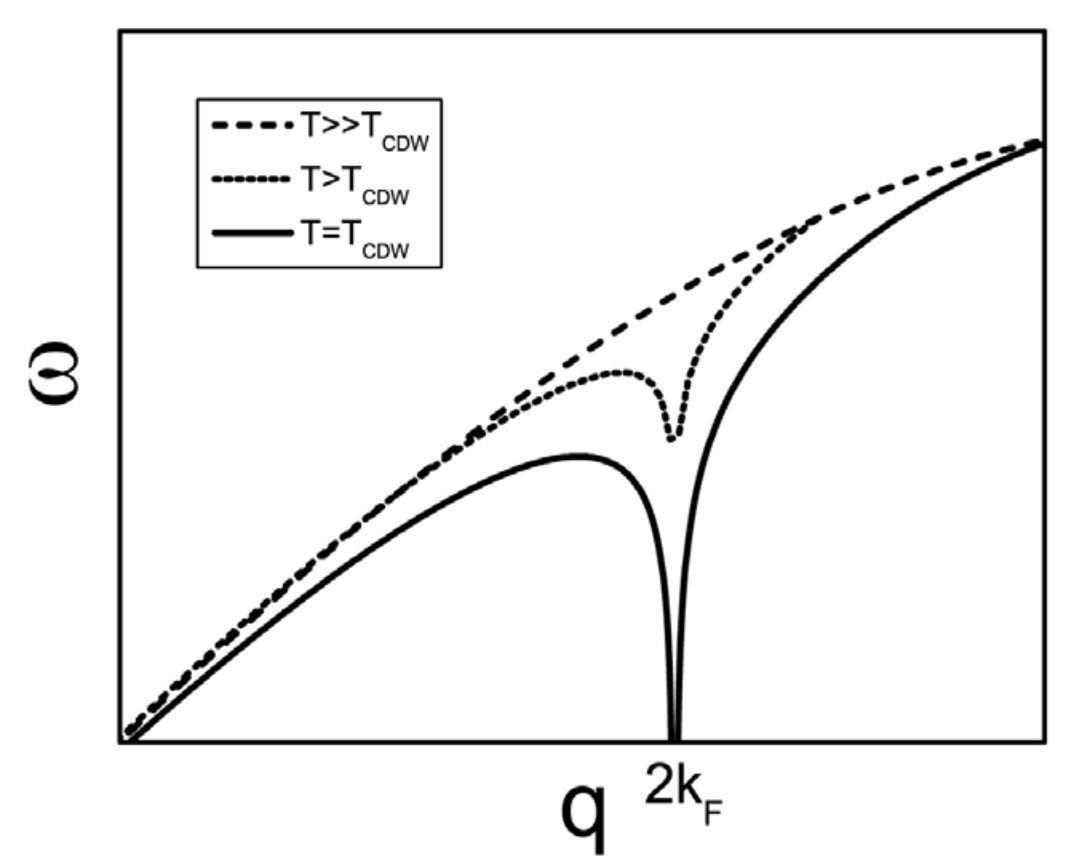
\includegraphics[width=2in]{figs/kohn_anomaly.png}
% % \caption{\label{fig:kohn_anomaly} Phonon energy of 1D chain at different $T$}
% % \end{figure}
% \end{itemize}
% \end{frame}

% \begin{frame}{Miao and Dean's \textit{Incommensurate Phonon Anomaly and the Nature of Charge Density Waves in Cuprates} (2018)}
% \begin{itemize}
% \item \textit{Goal:} Find unifying description for superconducting cuprates
% \item CDW instabilities are common superconducting cuprates
% \item CDWs have different ordering wave vectors
% \item They measured the $T$ dependence of the low-energy phonons in La$_{1.875}$Ba$_{0.125}$CuO$_4$ and compared it to YBa$_2$Cu$_3$O$_{6 + \delta}$
% \end{itemize}
% \end{frame}

% \begin{frame}{Inelastic x-ray scattering measurement of $S(\vf{Q}, \omega)$}
% \begin{itemize}
% \item Why measured $S(\vf{Q}, \omega)$? ``Because they can" - Lucas
% % \item Dashed lines are calculated using DFPT with PBE functional
% % \begin{figure}
% % 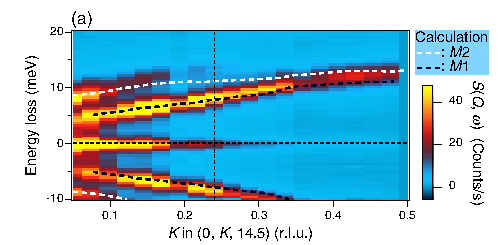
\includegraphics[width=3.5in]{figs/exp_sq.pdf}
% % \caption{\label{fig:exp_sq} Phonon dynamic structure factor at $T = 300~\mathrm{K}$}
% % \end{figure}
% \end{itemize}
% \end{frame}

% \begin{frame}{Example fits of spectra at $K$ = 0.09, 0.23, and 0.31 r.l.u. at different $T$}
% % \begin{figure}
% % 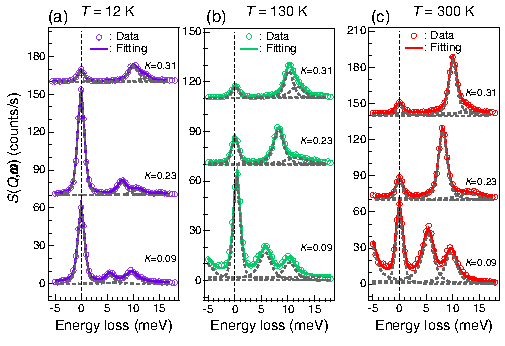
\includegraphics[width=3.5in]{figs/exp_fit.pdf}
% % \caption{\label{fig:exp_fit} }
% % \end{figure}
% \end{frame}

% \begin{frame}{Peaks at different $T$}
% % \begin{figure}
% % 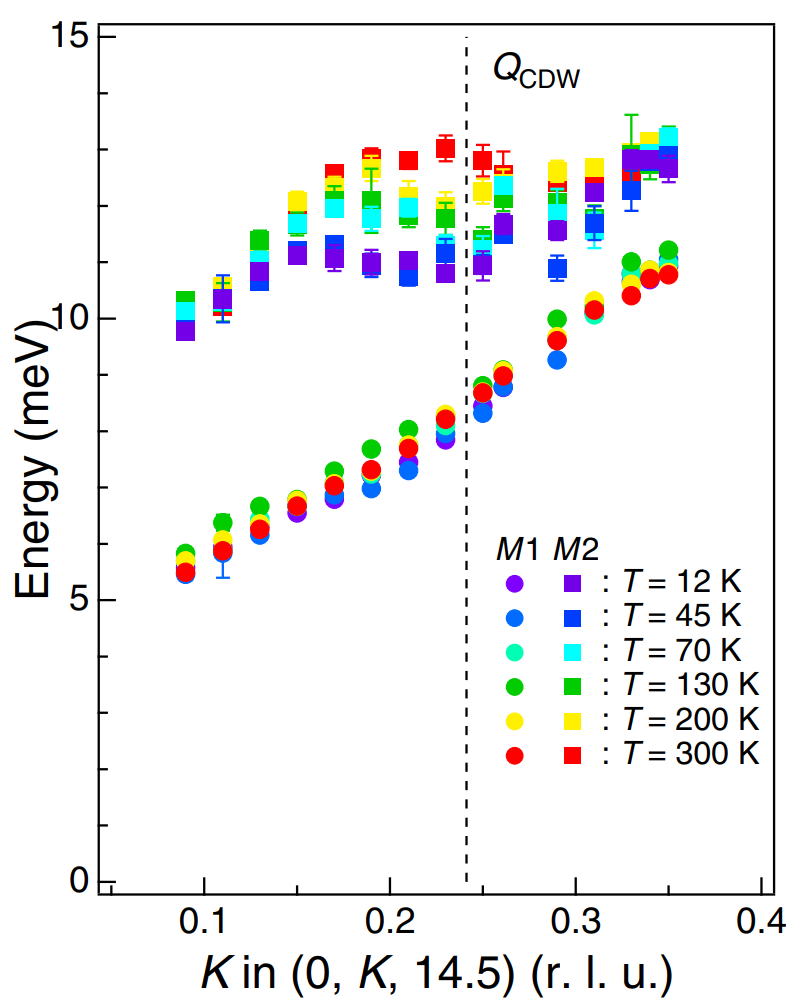
\includegraphics[width=2.2in]{figs/exp_E_k.png}
% % \caption{\label{fig:exp_E_k} $Q_{\text{CDW}} = 0.23~\mathrm{r.l.u.}$}
% % \end{figure}
% \end{frame}

% \begin{frame}{$T$ dependence at $K = 0.23~\mathrm{r.l.u.}$}
% \begin{itemize}
% \item Since they found that $M2$ has a large component of $c$-axis displacements, they suggest that $c$-axis coupled most strongly to the CDW
% % \begin{figure}
% % 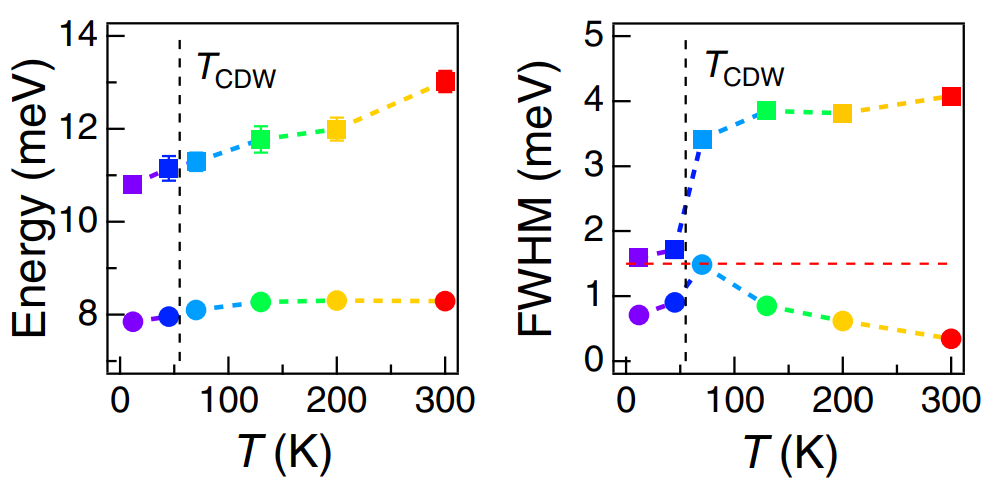
\includegraphics[width=3.5in]{figs/exp_T_dependence.png}
% % \caption{\label{fig:exp_T_dependence} $T_{\text{CDW}} = 55~\mathrm{K}$}
% % \end{figure}
% \end{itemize}
% \end{frame}

% \begin{frame}{Maximum phonon softening moves with increasing $T$}
% \begin{itemize}
% \item They conclude that $Q_{\text{CDW}} = 0.238~\mathrm{r.l.u.}$ at $T = 55~\mathrm{K}$, and $Q_{\text{CDW}} = 0.3~\mathrm{r.l.u.}$ at $T = 300~\mathrm{K}$
% \item Which is similar to a wave vector reported in YBa$_2$Cu$_3$O$_{6 + \delta}$
% % \begin{figure}
% % 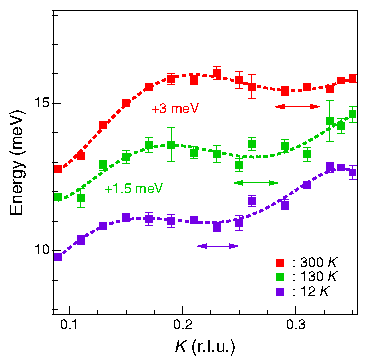
\includegraphics[width=2.5in]{figs/exp_E_k_zoomed.pdf}
% % \caption{\label{fig:exp_E_k_zoomed} }
% % \end{figure}
% \end{itemize}
% \end{frame}

% \begin{frame}{My research}
% \begin{itemize}
% \item \textit{Goal:} Identify phonon-softening modes of charge density waves in \ce{SrCuO2} and \ce{La2CuO4}???
% \item Step 1: Optimize the geometry of undoped and 1/4-doped \ce{SrCuO2} using DFT with 2x2 unit cells and PBEsol functional
% \item Step 2: Find phonon frequencies and eigenvectors at the gamma point
% \end{itemize}
% \end{frame}

% \begin{frame}{Identify how modes change after doping}
% \begin{itemize}
% \item The matrix element of $i$th AFM mode and $j$th Flip mode
% \begin{align}
% e_{ij} = \sum_{k = 1}^{48} v_{\text{AFM}, ik} \times v_{\text{Flip}, jk}
% \end{align}
% \item The two modes whose dot product is more than 0.8 are consider to be the same
% \begin{table}
% % \centering
% % \caption{\label{tab:dot} Dot products of  \ce{SrCuO2} (normallized within each column)}
% % \caption{\label{tab:widgets}Example values of the magnetic susceptibility, $\chi_v$.}
% \begin{tabular}{ccccccccccc}
% AFM / Flip & 1 & 2 & 3 & 4 & 5 & 6 & 7 & 8 & 9 & 10 \\
% % \colrule \\
% 1 & 0 & 0 & 0.895 & 0 & 0 & 0 & 0 & 0 & 0 & 0 \\
% 2 & 0.895 & 0 & 0 & 0 & 0 & 0 & 0 & 0 & 0 & 0 \\
% 3 & 0 & 0.875 & 0 & 0 & 0 & 0 & 0.001 & 0 & 0 & 0.047 \\
% 4 & 0 & 0 & 0 & 0.805 & 0 & 0 & 0 & 0 & 0 & 0 \\
% 5 & 0 & 0 & 0 & 0 & 0.806 & 0 & 0 & 0 & 0 & 0 \\
% 6 & 0 & 0 & 0 & 0 & 0 & 0 & 0 & 0 & 1.000 & 0 \\
% \end{tabular}
% \end{table}
% \end{itemize}
% \end{frame}

% \begin{frame}{The change in phonon frequency}
% % \begin{figure}
% % 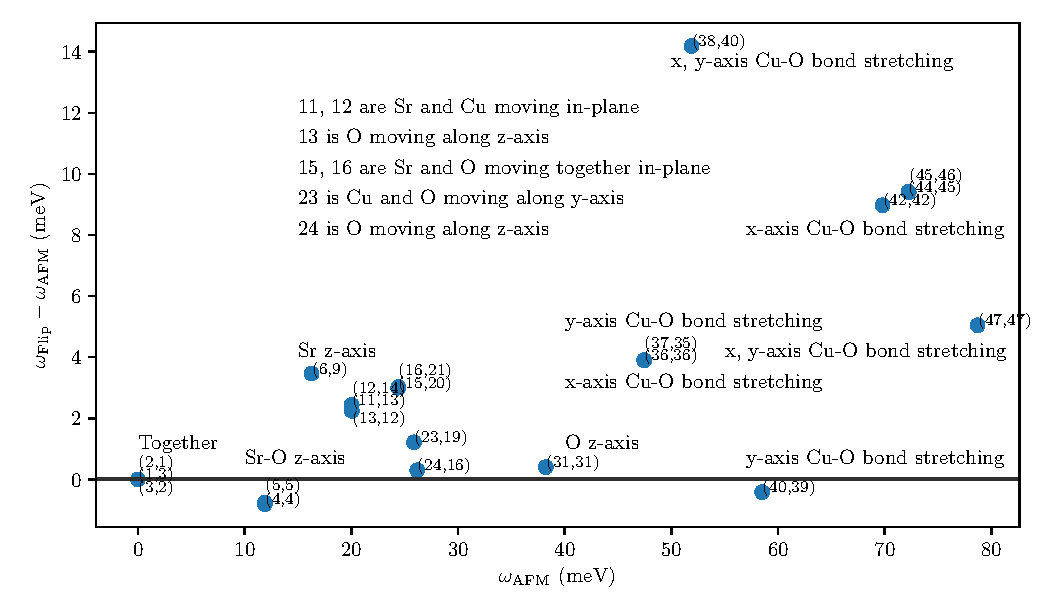
\includegraphics[width=4.2in]{figs/sco_afm_flip_freq.pdf}
% % \caption{\label{fig:sco_afm_flip_freq} See AVI files}
% % \end{figure}
% \end{frame}

% \begin{frame}{Conclusion}
% \begin{itemize}
% \item Kohn: Charge density waves affect phonon frequencies
% \item Dean: CDW in LCO and YBCO might be of the same origin (they both have $Q_{\text{CDW}} = 0.3~\mathrm{r.l.u.} at T = 300~\mathrm{K}$)
% \item My research: Doping weakens the Sr-O and Cu-O bonds
% \end{itemize}
% \end{frame}

\end{document}
